\documentclass[a4paper]{article}

%% Language and font encodings
\usepackage[english]{babel}
\usepackage[T1]{fontenc}

%% Sets page size and margins
\usepackage[a4paper,top=3cm,bottom=2cm,left=3cm,right=3cm,marginparwidth=1.75cm]{geometry}

%% Useful packages
\usepackage{amsmath}
\usepackage{graphicx}
\usepackage[colorinlistoftodos]{todonotes}
\usepackage[colorlinks=true, allcolors=blue]{hyperref}

\usepackage{graphics}
\usepackage{epsfig} 
\usepackage{mathptmx} 
% \usepackage{times} 
\usepackage{amssymb}
\usepackage{array}
\usepackage{subcaption}

\title{\date{\vspace{-5ex}}
Homework 1 - Basic Convolution \\
}



\begin{document}
\maketitle
\thispagestyle{empty}
\pagestyle{empty}


\section{Convolution (2 points)}
Recall the definition of convolution, 
\begin{align}
g = I \otimes f &\  
\end{align}
where \emph{\textbf{I}} and \emph{\textbf{f}} represents the image and kernel respectively. \\
\\Typically, when kernel $f$ is a 1-D vector, we get
\begin{align}
g(i) = \sum_{m}I(i - m)f(m) 
\end{align}
where $i$ is the index in the 1-D dimension.\\
\\If the kernel $f$ is a 2-D kernel, we have
\begin{align}
g(i, j) = \sum_{m, n}I(i - m, j - n)f(m, n) 
\end{align}
where $i$ and $j$ are the row and column indices respectively.\\
\\In this section, you need to perform the convolution \textbf{by hand}, get familiar with convolution in both 1-D and 2-D as well as its corresponding properties. \\
\\ \emph{\textbf{Note:}} All convolution operations in this section follow except additional notifications: 1. Zero-Padding, 2. Same Output Size, 3. An addition or multiplication with 0 will count as one operation.\\
\\For this problem, we will use the following $3 \times 3$ image:
\begin{equation}
I = 
	\begin{bmatrix}
	0.0 & 1.0 & -1.0 \\
    2.0 & 1.0 & 0.0 \\ 
    0.0 & 3.0 & -1.0 \\
	\end{bmatrix}
\end{equation}
You are given two 1-D vectors for convolution:
\begin{align}
f_{x} = 	
	\begin{bmatrix}
	-1.0 & 0.0 & 1.0 \\
	\end{bmatrix}\\
f_{y} = 	
	\begin{bmatrix}
	1.0 & 1.0 & 1.0 \\
	\end{bmatrix}^T
\end{align}\\
Let \( g_{1} = I \otimes f_{x} \otimes f_{y}\), \( f_{xy} = f_{x} \otimes f_{y}\) and \( g_{2} = I \otimes f_{xy}\).\\
\\ \emph{\textbf{Note:}} \( f_{xy}\) should be of full output size.
\begin{itemize}
\item \textbf{Question 1.1:} Compute \( g_{1}\) and \( g_{2}\) (At least show two steps for each convolution operation and intermediate results), and verify the associative property of convolution.

\item \textbf{Question 1.2:} How many operations are required for computing \( g_{1}\) and \( g_{2}\) respectively? 
addition and multiplication times in your result.

\item \textbf{Question 1.3:} What does convolution do to this image?
\end{itemize}




\newpage
\section{Kernel Estimation (2 points)}

Recall the special case of convolution discussed in class: The Impulse function. Using an impulse function, it is possible to 'shift' (and sometimes also 'scale') an image in a particular direction.\\
\\For example, when the following image 
\begin{equation}
I = 
	\begin{bmatrix}
    		     a & b & c \\
    		     d & e & f \\
    		     g & h & i 
	   		   \end{bmatrix}
\end{equation}
is convolved with the kernel, 
\begin{equation}
f = 
	\begin{bmatrix}
    		     1 & 0 & 0 \\
    		     0 & 0 & 0 \\
    		     0 & 0 & 0 
	   		   \end{bmatrix}
\end{equation}
it results in the output:
\begin{equation}
g = 
	\begin{bmatrix}
    		     e & f & 0 \\
    		     h & i & 0 \\
    		     0 & 0 & 0 
	   		   \end{bmatrix}
\end{equation}\\
\\Another useful trick to keep in mind is the decomposition of a convolution kernel into scaled impulse kernels. For example, a kernel
\begin{equation}
f = 
	\begin{bmatrix}
    		     0 & 0 & 7 \\
    		     0 & 0 & 0 \\
    		     0 & 4 & 0 
	   		   \end{bmatrix}
\end{equation}
can be decomposed into
\begin{center}
	$f_{1}$ = $7*\begin{bmatrix}
    		     0 & 0 & 1 \\
    		     0 & 0 & 0 \\
    		     0 & 0 & 0 
	   		   \end{bmatrix}$ \text{and}
    $f_{2}$ =   $4*\begin{bmatrix}
    		     0 & 0 & 0 \\
    		     0 & 0 & 0 \\
    		     0 & 1 & 0 
	   		   \end{bmatrix}$
\end{center}
\hspace{6pt}
\begin{itemize}
\item \textbf{Question:} Using the two tricks listed above, estimate the kernel $f$ \textbf{by hand} which when convolved with an image 
\begin{equation}
I = 
	\begin{bmatrix}
    		     1 & 5 & 2 \\
    		     7 & 8 & 6 \\
    		     3 & 9 & 4 
	   		   \end{bmatrix}
\end{equation}
results in the output image
\begin{equation}
g = 
	\begin{bmatrix}
    		     29 & 43 & 10 \\
    		     62 & 52 & 30 \\
    		     15 & 45 & 20 
	   		   \end{bmatrix}
\end{equation}
\end{itemize}
\textit{Hint: Look at the relationship between corresponding elements in g and I.}





\newpage
\section{Edge Moving (2 points)}
Object Recognition is one of the most popular applications in Computer Vision. The goal is to identify the object based on a template or a specific pattern of the object that has been learnt from a training dataset. Suppose we have a standard template for a "barrel" which is a $3 \times 3$ rectangle block in a $4 \times 4$ image. We also have an input $4 \times 4$ query image. Now, your task is to verify if the image in question contains a barrel. After preprocessing and feature extraction, the query image is simplified as $I_{Q}$ and the barrel template is $I_{T}$.
\[ I_{Q}=  \begin{bmatrix}
1 & 1 & 1 & 0 \\
1 & 1 & 1 & 0 \\
1 & 1 & 1 & 0 \\
0 & 0 & 0 & 0 \end{bmatrix}, I_{T}= \begin{bmatrix}
0 & 0 & 0 & 0 \\
0 & 1 & 1 & 1 \\
0 & 1 & 1 & 1 \\
0 & 1 & 1 & 1 \end{bmatrix} \]
Instinctively, the human eye can automatically detect a potential barrel in the top left corner of the query image but a computer can't do that right away. Basically, if the computer finds that the difference between query image's features and the template's features are minute, it will prompt with high confidence: 'Aha! I have found a barrel in the image'. However, in our circumstance, if we directly compute the pixel wise distance $D$ between $I_{Q}$ and $I_{T}$ where
\begin{eqnarray}
D(I_{Q}, I_{T}) = \sum_{i, j}(I_{Q}(i, j)- I_{T}(i, j))^2
\end{eqnarray}
we get $D = 10$ which implies that there's a huge difference between the query image and our template. To fix this problem, we can utilize the power of the convolution.
Let's define the 'mean shape' image $I_M$ which is the blurred version of $I_Q$ and $I_T$. 
\[I_{M}= \begin{bmatrix}
0.25 & 0.5 & 0.5 & 0.25 \\
0.5 & 1 & 1 & 0.5 \\
0.5 & 1 & 1 & 0.5 \\
0.25 & 0.5 & 0.5 & 0.25 \end{bmatrix} \]

\begin{itemize}
\item \textbf{Question 3.1:} Compute two $3 \times 3$ convolution kernels $f_1$, $f_2$ \textbf{by hand} such that $I_Q \otimes f_1 = I_M$ and $I_T \otimes f_2 = I_M$ where $\otimes$ denotes the convolution operation. (Assume zero-padding)

\item \textbf{Question 3.2:} For a convolution kernel $f=(f_1 + f_2) / 2$, we define $I_{Q}' = I_{Q} \otimes f$ and $I_{T}' = I_{T} \otimes f$. Compute $I_{Q}'$, $I_{T}'$ and $D(I_{Q}', I_{T}')$ \textbf{by hand}. Compare it with $D(I_{Q}, I_{T})$ and briefly explain what you find. 
\end{itemize}

\newpage
\section{Match the Kernels (2 points)}
\begin{itemize}
\item \textbf{Question 4.1 Match the corresponding kernels for the output images.} 

\begin{figure}[h!]
\centering
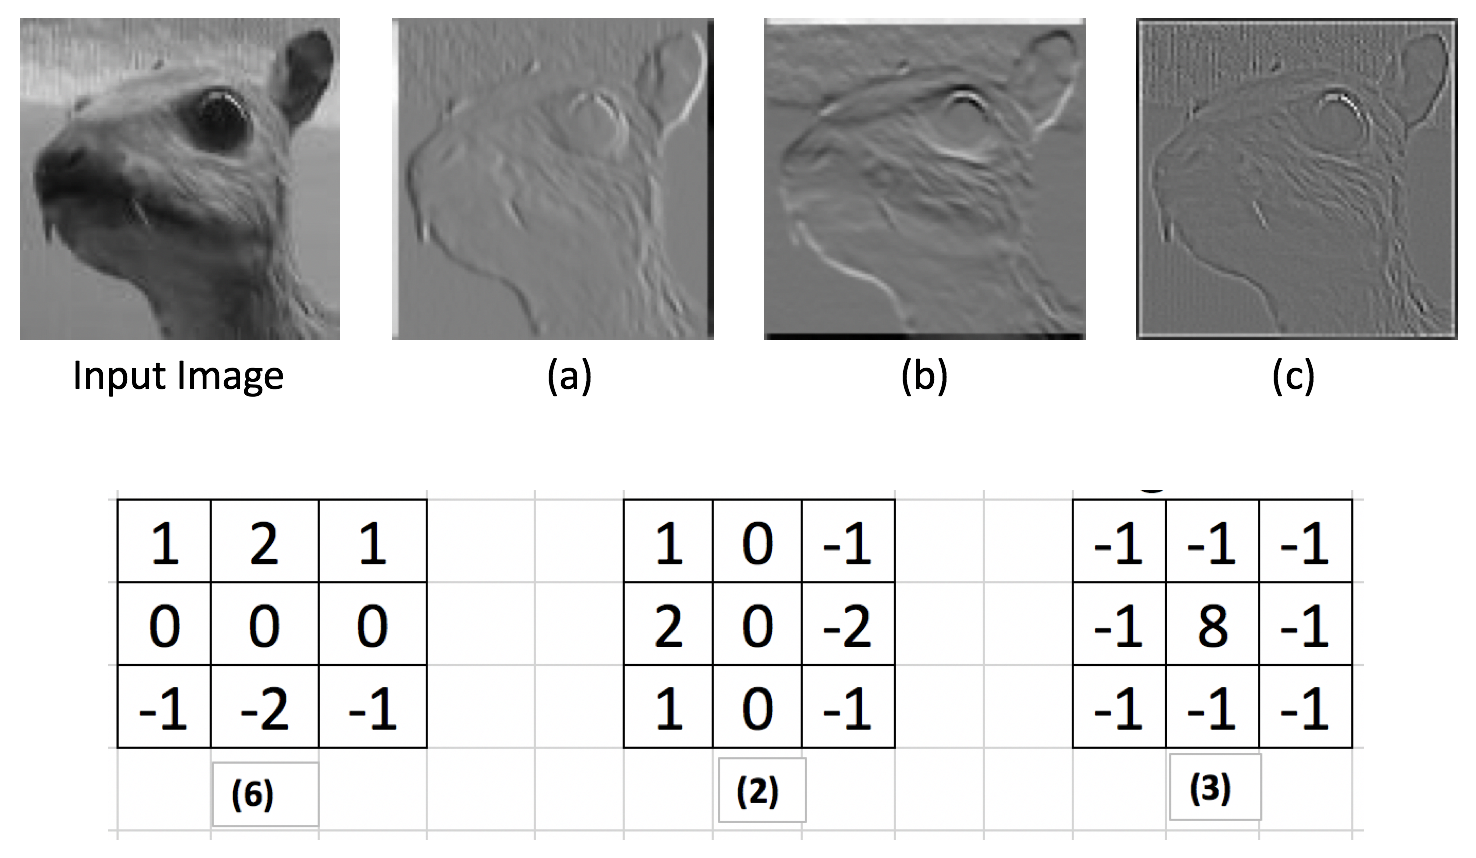
\includegraphics[width=\textwidth]{grayscale_conv.png}
\end{figure}



\item  \textbf{Question 4.2 Match the corresponding kernels for the output images.} 

\begin{figure}[h!]
\centering
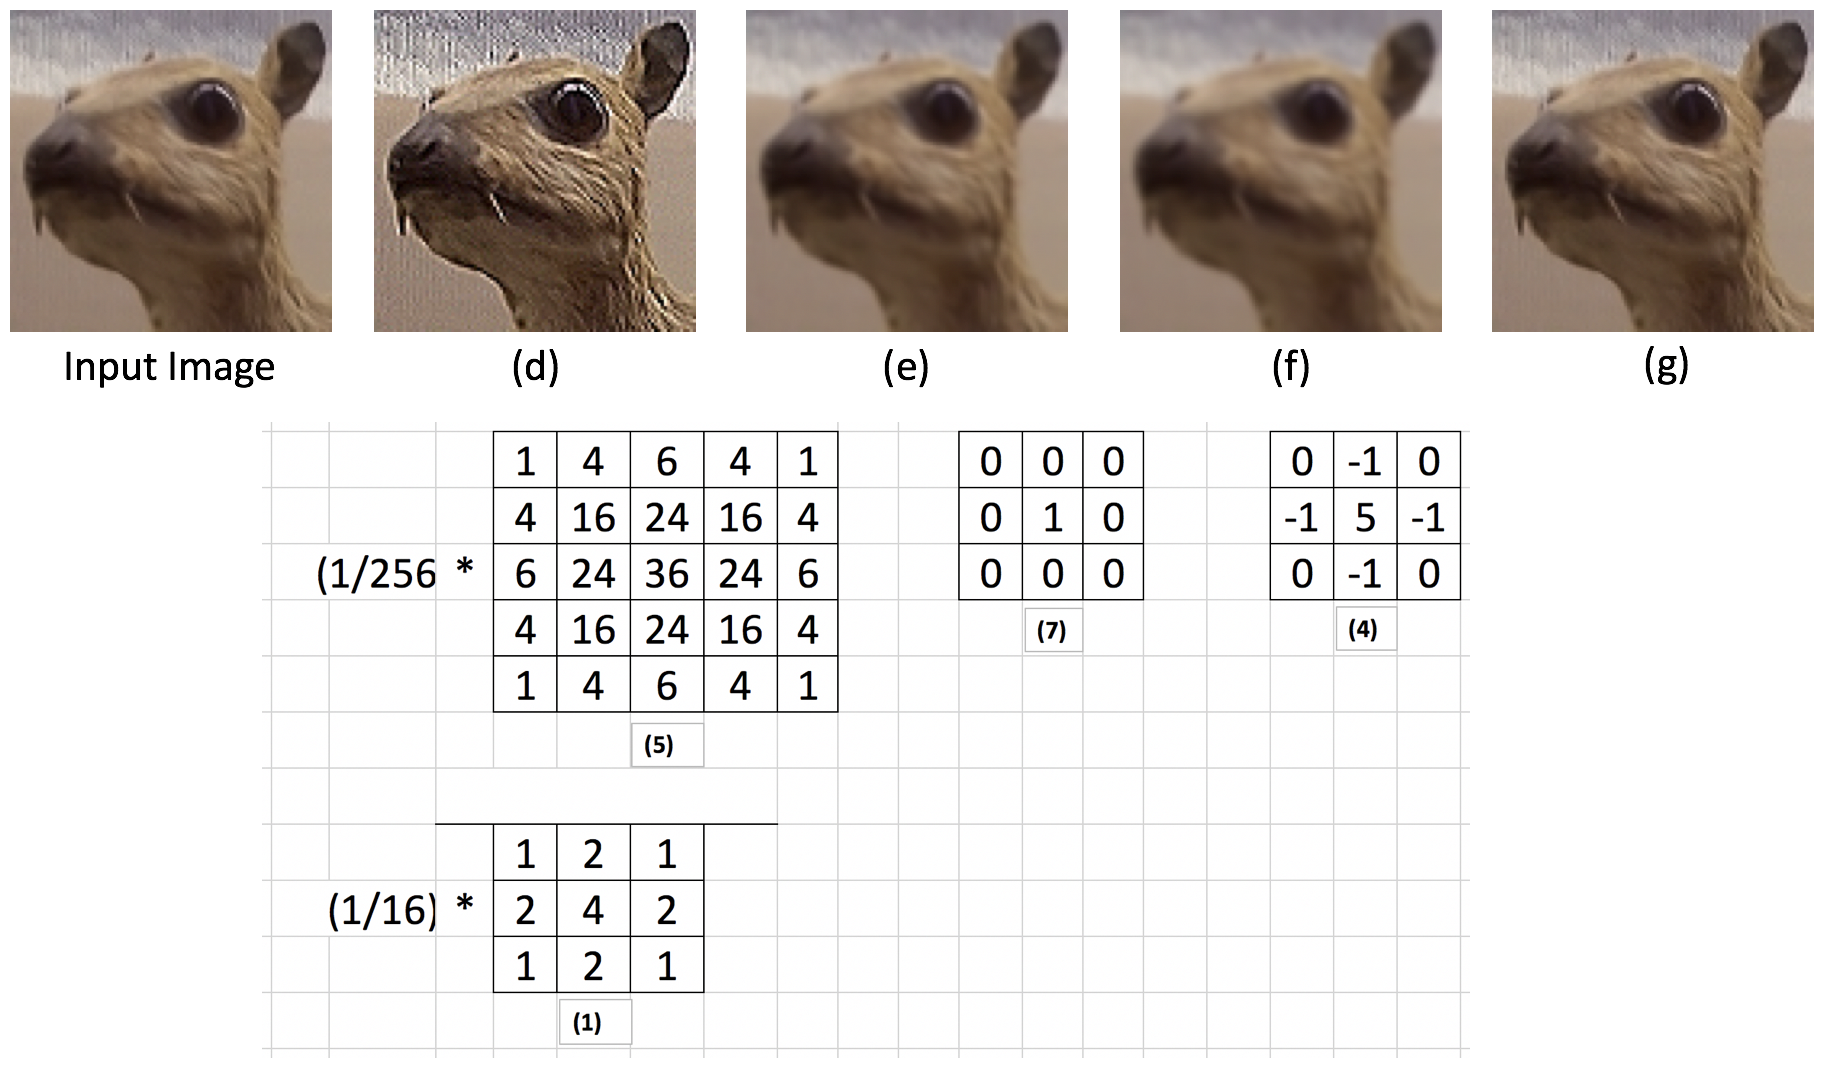
\includegraphics[width=\textwidth]{rgb_conv.png}
\end{figure}

\end{itemize}



\newpage
\section{Boundary Conditions (2 points)}

\\For this problem, we will use the following $3 \times 3$ image:
\begin{equation}
I = 
	\begin{bmatrix}
	1 & 1 & 1 \\
    1 & 3 & 2 \\ 
    1 & 1 & 1 \\
	\end{bmatrix}
\end{equation}
You are given 2-D convolution filter:
\begin{equation}
f = 
	\frac{1}{9}\begin{bmatrix}
	1 & 1 & 1 \\
    1 & 1 & 1 \\ 
    1 & 1 & 1 \\
	\end{bmatrix}
\end{equation}

\noindent Let \( g = I \underbrace{\otimes f\cdots \otimes f}_{\textrm{infinity times}}\). The output image $g$ has the same size as $I$.\\


\begin{itemize}
\item \textbf{Question 5.1:} When zero-padding is used, what's the output image $g$. (Give the verification process)
%\item \textbf{Question 5.1:} when padding with replication is used, what's the output image $g$.
\end{itemize}




\end{document}